\chapter{Introduction to EtherCAT}\label{sec:ecat_protocol}

As mentioned in the introduction, EtherCAT is an industrial Communication Profile developed by Beckhoff Automation GmbH that is 
standardized in the IEC 61588 under the RTE CPF. The development within this company is oriented to the use of 
open standards to increase its impact within the industry, but not only reduced to it but the overall smart cities field, in
a certain degree this approach eliminates the need for many expensive \emph{black boxes} as mentioned in ~\cite{beckhoff_automation}. %%Beckhoff_Urban_Automation_2013_e almost the introduction thing 
This implies that the interoperability of devices is almost guaranteed, at least from the specification perspective,
not only for private development centers but also for any other developer that follow the standards; if the standards 
are of public access, then this is a mean of empowerment of any group that might be willing
to create its own industrial-compatible technologies.

The OSADL emphasized in 2008, see article in ~\cite{beckhoff_vs_osadl}, for example, a vision for leading the integration
of open source in the industry by using the Linux Kernel as a certified Industrial RT (IRT) operative system for industrial embedded applications. 
Back in that day, Beckhoff Automation was involved in that discussion representing the contrary model. Nonetheless, in the last months the same company has
apparently retaken the open source initiative by the introduction of the FreeBSD compatible version of the TwinCAT Runtime---visit this newsletter ~\cite{beckhoff_freebsd}.%https://www.heise.de/newsticker/meldung/Open-Source-trifft-die-Industrie-201855.html
%**https://www.beckhoff.com/english.asp?highlights/twincat-bsd/default.htm

In comparison with other RTE profiles, EtherCAT has shown a higher performance, more flexible topology and lower costs than other field bus 
technologies. This  protocol  applies  a  master-slave  mode,  in  which  the  master  
device  uses  standard  100BASE-TX  Ethernet  adapter  and  the  EtherCAT  Slave  Controller (ESC), that implements an EtherCAT IP 
(intellectual property) core within an ASIC or an FPGA to process the frames. As  the  working  cycle starts, the  Master  
publishes a frame encapsulated a standardized 8802.3 frame. When it reaches an ESC, it analyses the address and location on the frame, decides
which parts of it are useful sections and then reads or writes data on it. As the
read-write operation finishes, the Working Counter (WKC) at the end of the frame is added by one, this way the data on the frame has been processed. 
This cycle repeats for each ESC within the topology. %Motion Control System using SERCOS over EtherCAT

EtherCAT supports almost all kinds of topology structure, such as ring, line, star and tree. The transmission speed of the interface is fixed to \SI{100}{\mega\bit\per\second}
with  full  duplex  communication.  The  network  is  able  to  connect  maximally 65535  devices  via  switch  and  media  converter.  
The  EtherCAT  system  can  update  1000  I/Os  in  just  \SI{30}{\micro\second} or  exchange \SI{1486}{\byte} contents in  \SI{300}{\micro\second}.
The previous technical data can be reviewed in ~\cite{beckhoff_datasheet} and an overview of the protocol in ~\cite{ecat_sercos}. %Motion Control System using SERCOS over EtherCAT

Important to highlight is that other CPs are also integrated as services inside the protocol, as mentioned before for 
the SERCOS specification in Sect.~\ref{sec:applications}. 
Other examples of these integrated CPs are File over EtherCAT (FoE) or Ethernet over EtherCAT (EoE), which  
make possible support a wide variety of devices and application layers in the same network.
A complete list of the communication profiles that are on hand
through the protocol's mailbox is given below, as to the overall layered integration can be seen in Fig.~\ref{fig:ecatprofiles}.
\begin{itemize}
    \item CoE: CAN application protocol over EtherCAT
    \item SoE: Servo drive profile, according to IEC 61800-7-204 (SERCOS protocol)
    \item EoE: Ethernet over EtherCAT
    \item FoE: File Access over EtherCAT (HTTP,FTP,etc)
    \item AoE: Automation Device Protocol over EtherCAT (ADS over EtherCAT)
\end{itemize}

\begin{figure}[ht]
    \centering
    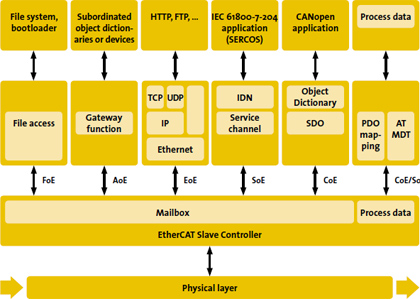
\includegraphics[width=.65\textwidth]{imgs/intro-ecatprofiles.jpg}
    \caption{Different communication profiles can coexist in the same system. Source from ~\cite{beckhoff_compatibility}.}
    \label{fig:ecatprofiles}
\end{figure}

An EtherCAT device with switch port properties using EoE would be the equivalent of the TSN compliant
switches, since they would insert any non time-sensitive TCP/IP fragment into the RTE traffic preventing
in this way the real time properties from being affected. Furthermore, the architecture of the protocol itself and
its early cooperation with the IEEE 802.1 group and the OPC Group ensure its continuous compatibility with the
standardization of TSN, OPC UA and the IoT paradigm. See the following article about compatibility \cite{beckhoff_compatibility}.%https://www.ethercat.org/en/technology.html#1.12


% *Add the image of the Ethernet frame having the EtherCAT datagram inside.
% *Explain the XAE tool and the PDI meaning
% *Quote maybe from paper section BASICS OF ETHERCAT AND PROFINET IRT Network Delay Analysis of EtherCAT and PROFINET IRT Protocols***
%** Question. What would happen if the synchronization mode within an EtherCAT network wants to be integrated to those of a TSN???


\begin{figure}[ht]
    \centering
    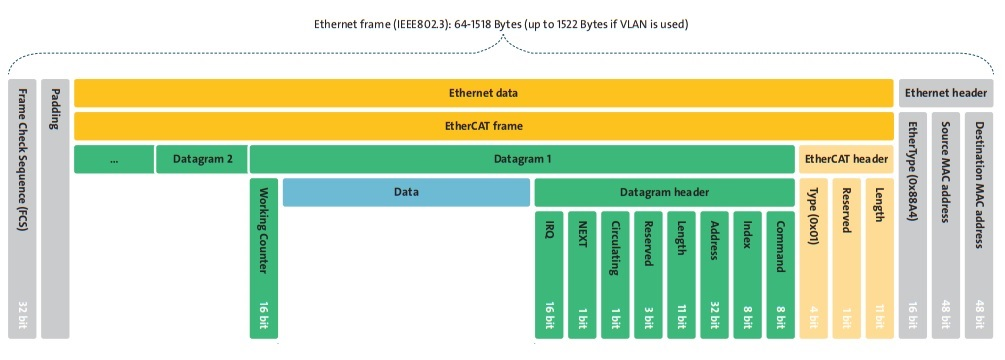
\includegraphics[width=\textwidth]{imgs/impl-dataframe.jpg}
    \caption{EtherCAT datagram within the Ethernet frame. Source from ~\cite{beckhoff_datalink}.}
    \label{fig:dataframe}
\end{figure}

\subsubsection{The data frame and the Synchronization Managers}\label{sec:synch_managers}

Besides the challenge of setting up the hardware and basic firmware for a correct data transmission between ESC and the host MCU; the description of the EtherCAT 
Slave device is a task that demands, at least, a basic understanding of the data frame exchange and how the protocol demands its synchronization. From here on, the following
topics are going to be summarized: Synchronization modes and managers.
Whenever there are Real Time constraints, and the device takes part of a control loop, synchronization modes are needed to be set correctly between the Master and
any Device present. For this task the Distributed Clocks (DC) are need to be synchronized. See the section 20 in ~\cite{beckhoff_enhancements}. %ETG.1020 - Synchronization and ETG.2000 - DC

There are three synchronization modes:  
\begin{description}
    \item[Free Run] Application is triggered by local clock and runs independently of EtherCAT cycle. 
    \item[SM-Synchronous] Application is synchronized whenever there are process data being written to the Synchronization Manager 2 (SM2).
    Moreover, any event generated by the Master is mapped onto an internal register or physically triggering an IRQ Pin of the ESC. 
    \item[DC-Synchronous] Within this synchronization mode the frame jitter can be even reduced down to \si{\nano\second} and use two different synchronization
    units within the ESC, namely the SM2 and SYNC/LATCH UNIT. 
\end{description}


\begin{figure}[ht]
    \centering
    \subfigure[Free Run]{\label{subfig:syncm1}{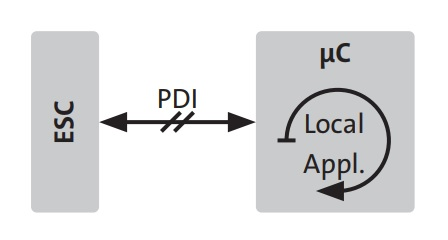
\includegraphics[width=0.3\textwidth]{imgs/impl-sync1.jpg}}}\hfill
    \subfigure[SM-Synchronization]{\label{subfig:syncm2}{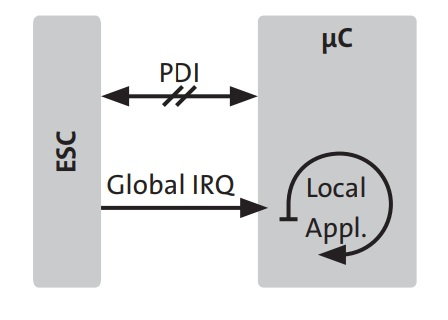
\includegraphics[width=0.3\textwidth]{imgs/impl-sync2.jpg}}}\hfill
    \subfigure[DC-Synchronization modes]{\label{subfig:syncm3}{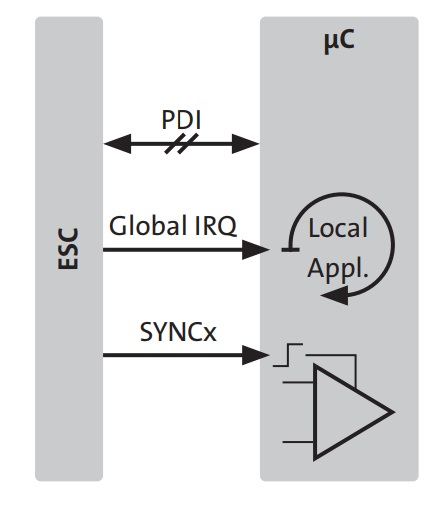
\includegraphics[width=0.3\textwidth]{imgs/impl-sync3.jpg}}}
    \caption{Synchronization modes. Definitions can be reviewed in depth within ~\cite{beckhoff_overview}.} %EtherCAT Device Protocol poster from EtherCAT resources
    \label{fig:syncmodes}
\end{figure} 

Synchronization Managers 1,2,3---as many as the hardware includes---(sometimes referred as SMXs) coordinate access to the ESC 
memory from both sides, Master and
Host MCU through the Process Data Interface (PDI). In case of process data communication it ensures that process data objects (PDO) 
can
always be written to the memory by EtherCAT and can always be read in the PDI side and vice versa (3-buffer mode). 
SyncManager 2/3 length is equal
to the Data Object lengths defined for receive and transmit data chunks respectively. SyncManagers are explained in detail in ~\cite{beckhoff_datalink}. %ETG.1000.4 Sync manager
The mapping of the process data objects within the Ethernet Frame can be seen in figure \ref{fig:dataframe} and \ref{fig:pdomapping}.
The correct setup of the SMXs ensure the consistency of the data and needs to be linked correctly depending on the characteristics of each ESC type,
 and SW Stack that are being used, this information is also linked to the CoE Object Dictionary (OD) and EtherCAT Slave Information (ESI) file.
\begin{figure}[ht]
    \centering
    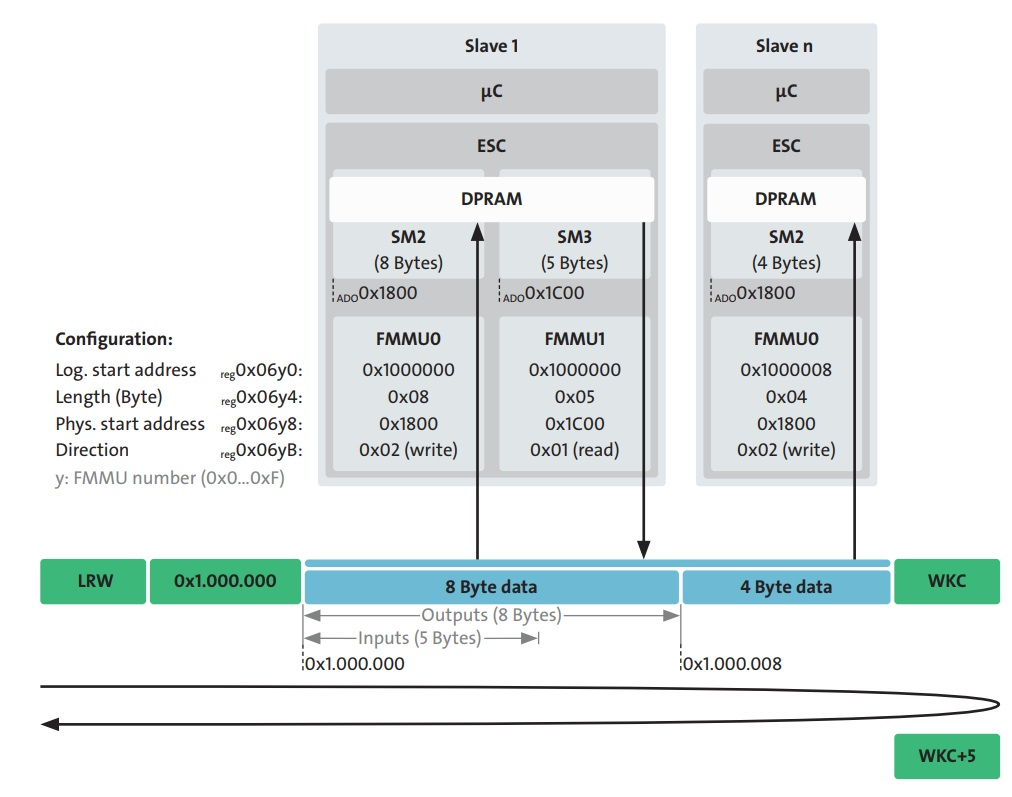
\includegraphics[width=.85\textwidth]{imgs/impl-dataframe_pdo.jpg}
    \caption{Depending on the different states of the Slave, there will be different data frames being exchanged with the Master. 
    The above one corresponds to the PDO which is updated continuously by the SM2/3 during Operation State (OP). Resource from SDO section in ~\cite{beckhoff_applayer}.}
    \label{fig:pdomapping}
\end{figure}